\documentclass[12pt]{article}

\usepackage[russian]{babel}
\usepackage{hhline}
\usepackage{graphicx}

\graphicspath{{pictures/}}
\DeclareGraphicsExtensions{.png}
\usepackage{multirow}
\usepackage{amsmath}
\usepackage{mathtext}
\usepackage[T2A]{fontenc}
\usepackage[utf8]{inputenc}
\usepackage{pscyr} 
\usepackage[left=1cm,right=1.5cm, top=1cm,bottom=1cm,bindingoffset=0cm]{geometry}
\begin{document}

\pagestyle{empty}
\begin{center}
\large{\textbf{Университет ИТМО}}
\end{center}
\rule{550pt}{1pt}
\par\bigskip\par\bigskip\par\bigskip\par\bigskip\par\bigskip\par\bigskip\par\bigskip\par\bigskip\par\bigskip\par\bigskip\par\bigskip\par\bigskip\par\bigskip\par\bigskip\par\bigskip\par\bigskip\par\bigskip
\par\bigskip\par\bigskip\par\bigskip\par\bigskip\par\bigskip\par\bigskip
\begin{center}
\Large
\textbf{Отчёт по лабораторной работа №2}

\textbf{\textit{«Изучение электронного осциллографа»}}


\end{center}
\par\bigskip\par\bigskip\par\bigskip\par\bigskip\par\bigskip\par\bigskip\par\bigskip\par\bigskip\par\bigskip\par\bigskip\par\bigskip\par\bigskip\par\bigskip\par\bigskip\par\bigskip
\begin{flushright}
\large
Выполнил: Федюкович  С. А.
\par\bigskip
Факультет: МТУ “Академия ЛИМТУ”
\par\bigskip
Группа: S3100                       
\par\bigskip\par\bigskip\par\bigskip

\rule{150pt}{0.5pt}
\par\bigskip\par\bigskip\par\bigskip\par\bigskip                                                            
 Проверил: Пшеничнов В. Е.
\par\bigskip \par\bigskip

\rule{150pt}{0.5pt}
\end{flushright}
\par\bigskip\par\bigskip\par\bigskip\par\bigskip\par\bigskip\par\bigskip\par\bigskip\par\bigskip\par\bigskip\par\bigskip     
\begin{center}
\large
Санкт-Петербург
\par\bigskip
2018
\end{center}
\newpage
\section*{Цель работы}
Ознакомление с устройством и работой электронного осциллографа, измерение с помощью осциллографа амплитуды и частоты синусоидального сигнала, определение скважности прямоугольного импульса и наблюдение фигур Лиссажу.
\section*{Краткое теоретическое описание}
Электронный осциллограф – прибор, используемый для исследования быстропротекающих процессов, измерения электрических и не электрических величин. Осциллограф в первую очередь приспособлен для измерения напряжений, но в отличие от цифровых приборов позволяет наблюдать процесс изменения напряжения на участке цепи в зависимости от времени. Поэтому для измерения других физических величин требуется их преобразование в изменение напряжения.

Благодаря возможности измерять процессы, происходящие во времени осциллограф является незаменимым прибором для исследования формы электрических сигналов и часто удобен для измерения частоты, периода и фазовых сдвигов в цепях. Однако в отличие от специализированных приборов, таких как цифровой вольтметр, частотомер, фазометр измерения самих физических величин с помощью осциллографа нельзя выполнить с высокой точностью. Типичная погрешность при измерении напряжения, или периода составляет величину порядка 1 – 4\%. Поэтому обычно осциллограф используют для визуального наблюдения и оценочного измерения, точное измерение физической величины выполняют с помощью других приборов. По этой же причине осциллографы часто объединяют с цифровыми мультиметрами, например как в осциллографе С1-117/1.
\begin{center}
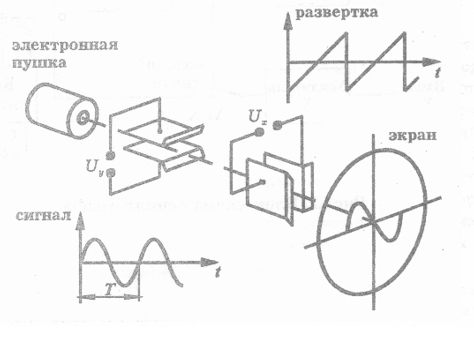
\includegraphics{img1}
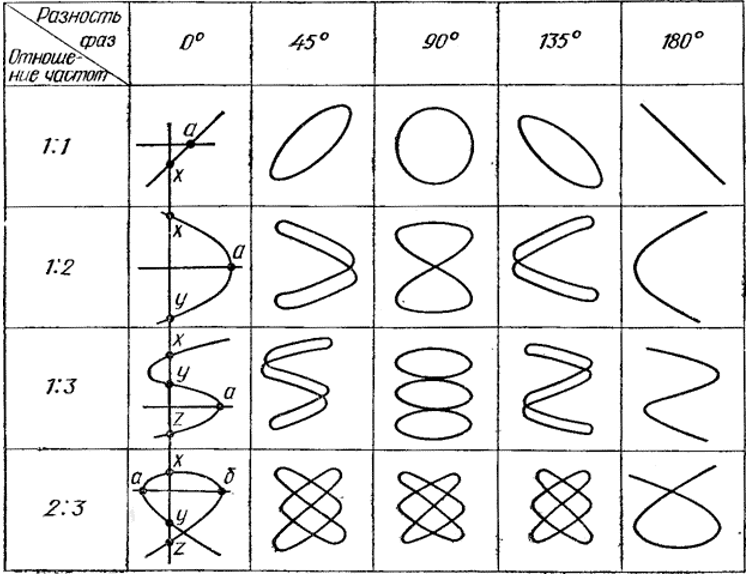
\includegraphics{img5}
\end{center}
\section*{Экспериментальные данные}
\begin{table}[h!]
\begin{center}
 Упражнение 1.

1 деление = $10мм$

\begin{tabular}{|c|c|c|c|c|c|c|c|c|c|}
\hline
$f_{ген}$, Гц & $U_{m}$, дел & $B$, дел & $T$, дел & мсек, дел & $U_{эфф}$, В & $U_{m}$, В & $T$, мс & $f=1/T$, кГц & $U_{m-эфф}, В$  \\
\hline
100 & 2,50 & 1 & 5,00 & 0,20 & 4,60 & 25 & 50 & 0,02 & 17,73\\
\hline
500 & 2,80 & 1 & 1,10 & 0,20 & 4,60 & 28 & 11 & 0,09 & 19,85\\
\hline
1000 & 2,70 & 1 & 0,50 & 0,20 & 4,59 & 27 & 5 & 0,20 & 19,14\\
\hline
\end{tabular}
\end{center}
\end{table}
\begin{table}[h!]
\begin{center}
 Упражнение 2.

\begin{tabular}{|c|c|c|c|}
\hline
$f_{факт}$, Гц & $T$, дел & $\tau$, дел & $T/\tau$\\
\hline
100 & 5,50 & 0,50 & 11,00 \\
\hline
500 & 1,10 & 0,40 & 2,75\\
\hline
\end{tabular}
\end{center}
\end{table}
\begin{center}
\newpage
Упражнение 3.

50 В

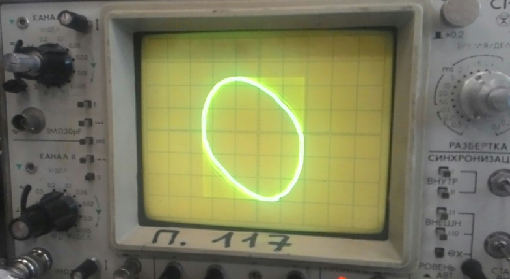
\includegraphics{img2}\\

100 В

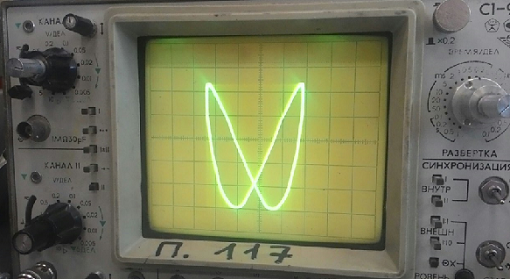
\includegraphics{img3}\\

250 В

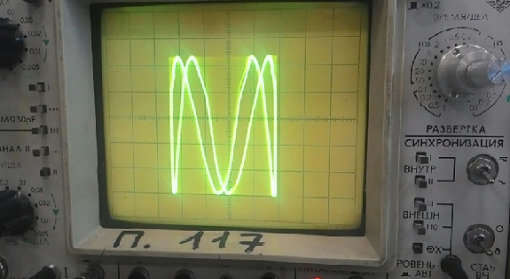
\includegraphics{img4}
\end{center}
\section*{Вывод}
В ходе выполнения данной лабораторной работы было выполнено ознакомление с устройством электронного осциллографа, с помощью которого, в последствии, производилось изучение процессов в простых электрических цепях, некоторые из которых наглядно были представлены в отчете лабораторной работы.
\end{document}